\documentclass[tikz,border=4pt]{standalone}
% Shared style for every figure and for the deck: one accent, one
% highlight, thin lines, rounded nodes, nothing decorative.
\usepackage[T1]{fontenc}
\usepackage{lmodern}
\renewcommand{\familydefault}{\sfdefault}
\usepackage{tikz}
\usetikzlibrary{arrows.meta,positioning,calc,shapes.misc,fit,backgrounds,decorations.pathreplacing}
\definecolor{ink}{RGB}{40,40,40}
\definecolor{soft}{RGB}{150,150,150}
\definecolor{faint}{RGB}{225,225,225}
\definecolor{accent}{RGB}{0,95,115}
\definecolor{accentlight}{RGB}{214,232,236}
\definecolor{warn}{RGB}{196,84,40}
\definecolor{warnlight}{RGB}{247,226,216}
\tikzset{
  every picture/.style={color=ink, line width=0.5pt, font=\small},
  node distance=12mm and 18mm,
  box/.style={draw=ink, rounded corners=2pt, fill=white, inner sep=5pt, minimum height=7mm, align=center},
  maker/.style={box, minimum width=18mm},
  cat/.style={box, inner sep=3.5pt, minimum height=6mm},
  root/.style={box, fill=accentlight, draw=accent},
  bad/.style={box, fill=warnlight, draw=warn},
  ghost/.style={box, draw=soft, text=soft, dashed},
  flow/.style={-{Stealth[length=4pt,width=3.5pt]}, line width=0.5pt},
  sub/.style={-{Stealth[length=4pt,width=3.5pt]}, line width=0.5pt, color=soft},
  strong/.style={flow, color=accent, line width=0.8pt},
  wrong/.style={flow, color=warn},
  lbl/.style={font=\footnotesize, text=ink, inner sep=1.5pt, fill=white},
  note/.style={font=\footnotesize, text=soft, align=center},
  rate/.style={font=\footnotesize, text=accent, inner sep=1pt, fill=white},
}

\usepackage{amsmath}
\usepackage{pgfplots}
\pgfplotsset{compat=1.17}

\begin{document}
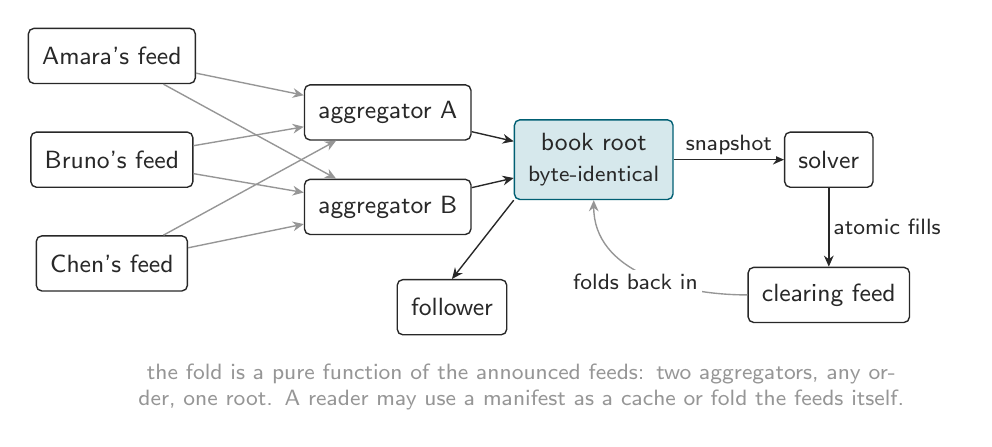
\begin{tikzpicture}[node distance=6mm and 14mm]
  \node[maker] (a) {Amara's feed};
  \node[maker, below=of a] (b) {Bruno's feed};
  \node[maker, below=of b] (c) {Chen's feed};
  \node[box, right=of b, yshift=6mm] (A) {aggregator A};
  \node[box, right=of b, yshift=-6mm] (B) {aggregator B};
  \node[root, right=16mm of $(A)!0.5!(B)$] (m) {book root\\{\footnotesize byte-identical}};
  \node[box, right=of m] (s) {solver};
  \node[box, below=10mm of s] (set) {clearing feed};
  \node[box, below=10mm of m, xshift=-18mm] (f) {follower};
  \foreach \x in {a,b,c} { \draw[sub] (\x) -- (A); \draw[sub] (\x) -- (B); }
  \draw[flow] (A) -- (m); \draw[flow] (B) -- (m);
  \draw[flow] (m) -- node[lbl, above] {snapshot} (s);
  \draw[flow] (s) -- node[lbl, right] {atomic fills} (set);
  \draw[sub] (set.west) to[out=180, in=-90] node[lbl, pos=0.55, below] {folds back in} (m.south);
  \draw[flow] (m.south west) -- (f.north);
  \node[note, text width=110mm] at (52mm,-42mm) {the fold is a pure function of the announced feeds: two aggregators, any order, one root. A reader may use a manifest as a cache or fold the feeds itself.};
\end{tikzpicture}
\end{document}
